\Chapter{A játék matematikai modellje}

A játék véletlentől függő elemeket tartalmaz, viszont a játékosokra nézve teljes információs. A játék menete véges állapotgéppel modellezhető. A leszűkített szabályrendszerre vonatkozó játékmenetet \aref{fig:flowchart}. ábra mutatja be.

\begin{figure}[h]
\centering
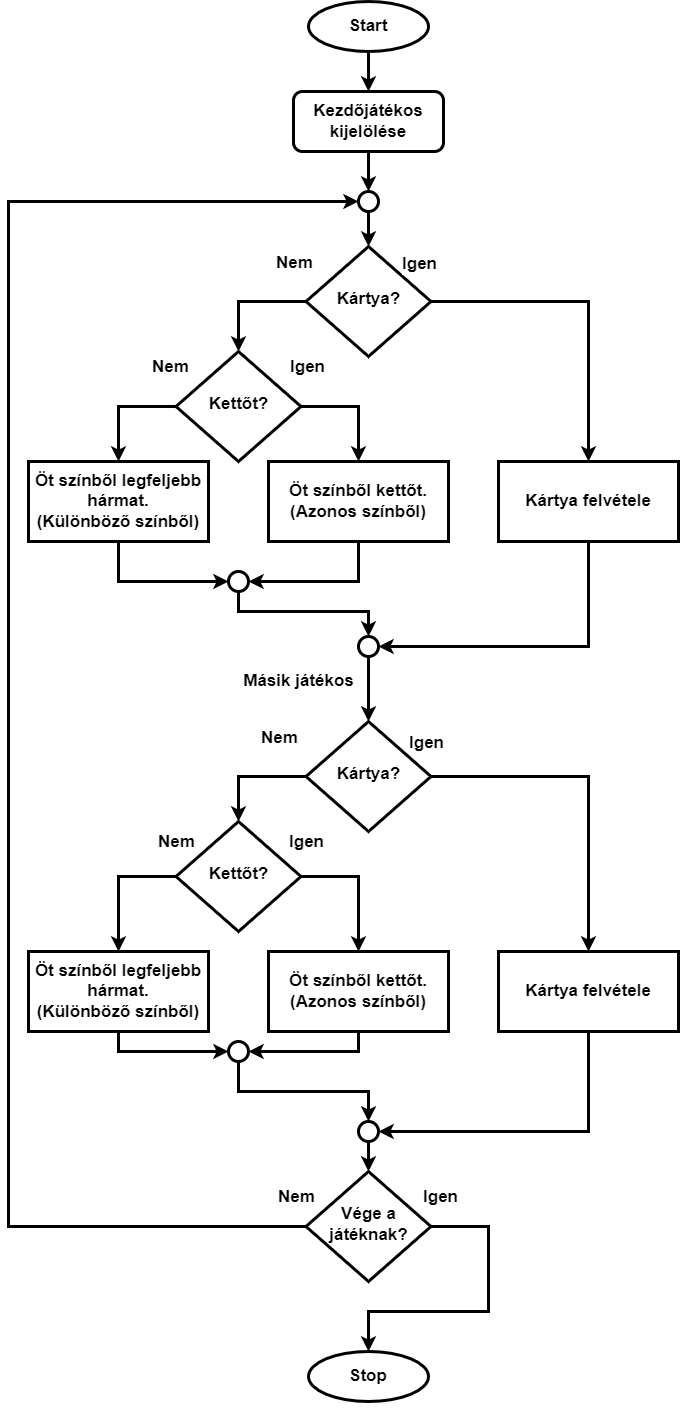
\includegraphics[scale=0.42]{images/flowchart.png}
\caption{A játék folyamatábrája.}
\label{fig:flowchart}
\end{figure}

Ahogy a folyamatábrán is látható a játék köreinek felépítése viszonylag egyszerűen zajlik. Kezdetben kijelöljük az éppen soron következő játékost, majd megkezdődik a köre. Először eldönti, hogy kártyát vagy zsetont szeretne választani az adott körben. Ha kártyát, akkor a kártyahúzás után vége a körének. Ha viszont zsetont, akkor két lehetőség áll a rendelkezésére: vagy hármat választ, egyet-egyet a különböző színekből, vagy pedig kettőt, de azonos színből. A két lehetőség valamelyikének végrehajtása után szintén átadja a kört a másik játékos számára, akinek ugyanezek a lehetőségek állnak a rendelkezésére. A második játékos köre végén megvizsgáljuk, hogy megvalósult-e a játék végét jelentő feltétel. Ha nem, akkor az első játékos köre kezdődik meg újra, és halad a folyamat a leírtak szerint, ha pedig igen, akkor a játék befejeződik.

A játékos természetesen csak a számára elérhető kártyákból és zsetonokból választhat. Egy zseton akkor elérhető a számára, ha abból legalább egy van a játéktéren, a kártya pedig akkor, ha a megvásárlásához szükséges zsetonok a birtokában vannak. Ezek a zsetonok lehetnek sima, korábban elvett zsetonok, vagy akár a kártyák korábbi megvásárlása nyomán megszerzett bónusz értékek.

A kártyalapok a játéktérre való elhelyezése randomizálva történik az adott szintű kártyapaklikból megfelelően. A kártyák szimmetrikusan szerepelnek a paklikban, így a zsetonok teljesen egyenértékűek a teljes kártyakészletet tekintve. A játék előrehaladtával és a kártyalapok fogyásával értelemszerűen folyamatosan változik ez az arány. A zsetonok értékei a játéktéren lent lévő lapok függvényében változik. Emellett az is változtatja a zsetonok felhúzásában való lehetőségeink számát, hogy a korábbi körökben miként alakul a lent lévő zsetonok száma, mivel kettőt egy színből csak akkor lehet húzni, ha ott legalább négy van a kör kezdetekor, ezen felül pedig csak azokból a színekből lehet választani, ahol van legalább egy zseton. A játék vége felé haladva a zsetonfelhúzás kissé értékét veszti, hiszen a kártyalapok ingyen megszerzése és ezáltal a mechanizmus építése nagyobb előnyökhöz juttatja a játékosokat.
